\documentclass[journal,12pt,twocolumn]{IEEEtran}
%
\usepackage{setspace}
\usepackage{gensymb}
%\doublespacing
\singlespacing

%\usepackage{graphicx}
%\usepackage{amssymb}
%\usepackage{relsize}
\usepackage[cmex10]{amsmath}
%\usepackage{amsthm}
%\interdisplaylinepenalty=2500
%\savesymbol{iint}
%\usepackage{txfonts}
%\restoresymbol{TXF}{iint}
%\usepackage{wasysym}
\usepackage{amsthm}
\usepackage{mathrsfs}
\usepackage{txfonts}
\usepackage{stfloats}
\usepackage{cite}
\usepackage{cases}
\usepackage{subfig}
%\usepackage{xtab}
\usepackage{longtable}
\usepackage{multirow}
%\usepackage{algorithm}
%\usepackage{algpseudocode}
\usepackage{enumitem}
\usepackage{mathtools}
\usepackage{iithtlc}
\usepackage{tikz}
\usepackage{circuitikz}
\usepackage{verbatim}
%\usepackage{stmaryrd}
\usepackage{tkz-euclide} % loads  TikZ and tkz-base
\usetkzobj{all}
\usepackage{listings}
%\usepackage{wasysym}
%\newcounter{MYtempeqncnt}
\DeclareMathOperator*{\Res}{Res}
%\renewcommand{\baselinestretch}{2}
\renewcommand\thesection{\arabic{section}}
\renewcommand\thesubsection{\thesection.\arabic{subsection}}
\renewcommand\thesubsubsection{\thesubsection.\arabic{subsubsection}}

\renewcommand\thesectiondis{\arabic{section}}
\renewcommand\thesubsectiondis{\thesectiondis.\arabic{subsection}}
\renewcommand\thesubsubsectiondis{\thesubsectiondis.\arabic{subsubsection}}

% correct bad hyphenation here
\hyphenation{op-tical net-works semi-conduc-tor}

\lstset{
language=tex,
frame=single, 
breaklines=true
}

\begin{document}
%


\newtheorem{theorem}{Theorem}[section]
\newtheorem{problem}{Problem}
\newtheorem{proposition}{Proposition}[section]
\newtheorem{lemma}{Lemma}[section]
\newtheorem{corollary}[theorem]{Corollary}
\newtheorem{example}{Example}[section]
\newtheorem{definition}[problem]{Definition}
%\newtheorem{thm}{Theorem}[section] 
%\newtheorem{defn}[thm]{Definition}
%\newtheorem{algorithm}{Algorithm}[section]
%\newtheorem{cor}{Corollary}
\newcommand{\BEQA}{\begin{eqnarray}}
\newcommand{\EEQA}{\end{eqnarray}}
\newcommand{\define}{\stackrel{\triangle}{=}}

\bibliographystyle{IEEEtran}
%\bibliographystyle{ieeetr}


\providecommand{\mbf}{\mathbf}
\providecommand{\pr}[1]{\ensuremath{\Pr\left(#1\right)}}
\providecommand{\qfunc}[1]{\ensuremath{Q\left(#1\right)}}
\providecommand{\sbrak}[1]{\ensuremath{{}\left[#1\right]}}
\providecommand{\lsbrak}[1]{\ensuremath{{}\left[#1\right.}}
\providecommand{\rsbrak}[1]{\ensuremath{{}\left.#1\right]}}
\providecommand{\brak}[1]{\ensuremath{\left(#1\right)}}
\providecommand{\lbrak}[1]{\ensuremath{\left(#1\right.}}
\providecommand{\rbrak}[1]{\ensuremath{\left.#1\right)}}
\providecommand{\cbrak}[1]{\ensuremath{\left\{#1\right\}}}
\providecommand{\lcbrak}[1]{\ensuremath{\left\{#1\right.}}
\providecommand{\rcbrak}[1]{\ensuremath{\left.#1\right\}}}
\theoremstyle{remark}
\newtheorem{rem}{Remark}
\newcommand{\sgn}{\mathop{\mathrm{sgn}}}
\providecommand{\abs}[1]{\left\vert#1\right\vert}
\providecommand{\res}[1]{\Res\displaylimits_{#1}} 
\providecommand{\norm}[1]{\lVert#1\rVert}
\providecommand{\mtx}[1]{\mathbf{#1}}
\providecommand{\mean}[1]{E\left[ #1 \right]}
\providecommand{\fourier}{\overset{\mathcal{F}}{ \rightleftharpoons}}
%\providecommand{\hilbert}{\overset{\mathcal{H}}{ \rightleftharpoons}}
\providecommand{\system}{\overset{\mathcal{H}}{ \longleftrightarrow}}
	%\newcommand{\solution}[2]{\textbf{Solution:}{#1}}
\newcommand{\solution}{\noindent \textbf{Solution: }}
\providecommand{\dec}[2]{\ensuremath{\overset{#1}{\underset{#2}{\gtrless}}}}
%\numberwithin{equation}{section}
%\numberwithin{problem}{section}
%\numberwithin{definition}{section}

\makeatletter
\@addtoreset{figure}{problem}
\makeatother

\let\StandardTheFigure\thefigure
%\renewcommand{\thefigure}{\theproblem.\arabic{figure}}
\renewcommand{\thefigure}{\theproblem}



\def\putbox#1#2#3{\makebox[0in][l]{\makebox[#1][l]{}\raisebox{\baselineskip}[0in][0in]{\raisebox{#2}[0in][0in]{#3}}}}
     \def\rightbox#1{\makebox[0in][r]{#1}}
     \def\centbox#1{\makebox[0in]{#1}}
     \def\topbox#1{\raisebox{-\baselineskip}[0in][0in]{#1}}
     \def\midbox#1{\raisebox{-0.5\baselineskip}[0in][0in]{#1}}

\vspace{3cm}

\title{
	\logo{
	School Mathematics through Python
	}
}
%\title{
%	\logo{Matrix Analysis through Octave}{\begin{center}\includegraphics[scale=.24]{tlc}\end{center}}{}{HAMDSP}
%}


% paper title
% can use linebreaks \\ within to get better formatting as desired
%\title{Matrix Analysis through Octave}
%
%
% author names and IEEE memberships
% note positions of commas and nonbreaking spaces ( ~ ) LaTeX will not break
% a structure at a ~ so this keeps an author's name from being broken across
% two lines.
% use \thanks{} to gain access to the first footnote area
% a separate \thanks must be used for each paragraph as LaTeX2e's \thanks
% was not built to handle multiple paragraphs
%

\author{G V V Sharma$^{*}$% <-this % stops a space
\thanks{*The author is with the Department
of Electrical Engineering, Indian Institute of Technology, Hyderabad
502285 India e-mail:  gadepall@iith.ac.in.}% <-this % stops a space
%\thanks{J. Doe and J. Doe are with Anonymous University.}% <-this % stops a space
%\thanks{Manuscript received April 19, 2005; revised January 11, 2007.}}
}
% note the % following the last \IEEEmembership and also \thanks - 
% these prevent an unwanted space from occurring between the last author name
% and the end of the author line. i.e., if you had this:
% 
% \author{....lastname \thanks{...} \thanks{...} }
%                     ^------------^------------^----Do not want these spaces!
%
% a space would be appended to the last name and could cause every name on that
% line to be shifted left slightly. This is one of those "LaTeX things". For
% instance, "\textbf{A} \textbf{B}" will typeset as "A B" not "AB". To get
% "AB" then you have to do: "\textbf{A}\textbf{B}"
% \thanks is no different in this regard, so shield the last } of each \thanks
% that ends a line with a % and do not let a space in before the next \thanks.
% Spaces after \IEEEmembership other than the last one are OK (and needed) as
% you are supposed to have spaces between the names. For what it is worth,
% this is a minor point as most people would not even notice if the said evil
% space somehow managed to creep in.



% The paper headers
%\markboth{Journal of \LaTeX\ Class Files,~Vol.~6, No.~1, January~2007}%
%{Shell \MakeLowercase{\textit{et al.}}: Bare Demo of IEEEtran.cls for Journals}
% The only time the second header will appear is for the odd numbered pages
% after the title page when using the twoside option.
% 
% *** Note that you probably will NOT want to include the author's ***
% *** name in the headers of peer review papers.                   ***
% You can use \ifCLASSOPTIONpeerreview for conditional compilation here if
% you desire.




% If you want to put a publisher's ID mark on the page you can do it like
% this:
%\IEEEpubid{0000--0000/00\$00.00~\copyright~2007 IEEE}
% Remember, if you use this you must call \IEEEpubidadjcol in the second
% column for its text to clear the IEEEpubid mark.



% make the title area
\maketitle

\newpage

\tableofcontents

\bigskip


%\begin{abstract}
%%\boldmath
%In this letter, an algorithm for evaluating the exact analytical bit error rate  (BER)  for the piecewise linear (PL) combiner for  multiple relays is presented. Previous results were available only for upto three relays. The algorithm is unique in the sense that  the actual mathematical expressions, that are prohibitively large, need not be explicitly obtained. The diversity gain due to multiple relays is shown through plots of the analytical BER, well supported by simulations. 
%
%\end{abstract}
% IEEEtran.cls defaults to using nonbold math in the Abstract.
% This preserves the distinction between vectors and scalars. However,
% if the journal you are submitting to favors bold math in the abstract,
% then you can use LaTeX's standard command \boldmath at the very start
% of the abstract to achieve this. Many IEEE journals frown on math
% in the abstract anyway.

% Note that keywords are not normally used for peerreview papers.
%\begin{IEEEkeywords}
%Cooperative diversity, decode and forward, piecewise linear
%\end{IEEEkeywords}



% For peer review papers, you can put extra information on the cover
% page as needed:
% \ifCLASSOPTIONpeerreview
% \begin{center} \bfseries EDICS Category: 3-BBND \end{center}
% \fi
%
% For peerreview papers, this IEEEtran command inserts a page break and
% creates the second title. It will be ignored for other modes.
%\IEEEpeerreviewmaketitle

\begin{abstract}
This manual shows how to generate figures encountered in high school geometry using python. The process provides simple applications
of coordinate geometry.
%The focus of this text is on investigating the properties of triangles and circles through coordinate geometry.  An early exposure to coordinate geometry allows students to use computers for mathematical visualizations and computing.  This book provides an alternative approach to geometry which may be useful to those having difficulties with traditional methods.  In the process, almost all the basic concepts of coordinate geometry are covered.  Instead of teaching geometry and coordinate geometry as separate subjects in high school, this textbook shows how to develop  a holistic approach for teaching math.
\end{abstract}

\section{Line}
\begin{problem}
\label{prob:draw_triangle}
Let
\begin{equation}
A =
\begin{pmatrix}
-2
\\
-2
\end{pmatrix},
B =
\begin{pmatrix}
1
\\
3
\end{pmatrix},
C =
\begin{pmatrix*}[r]
4
\\
-1
\end{pmatrix*}.
\end{equation}
Draw $\Delta ABC$.
\end{problem}
\solution
The following code yields the desired plot in Fig. \ref{fig:triangle_def}
\lstinputlisting{./codes/draw_triangle.py}
\begin{figure}
\centering
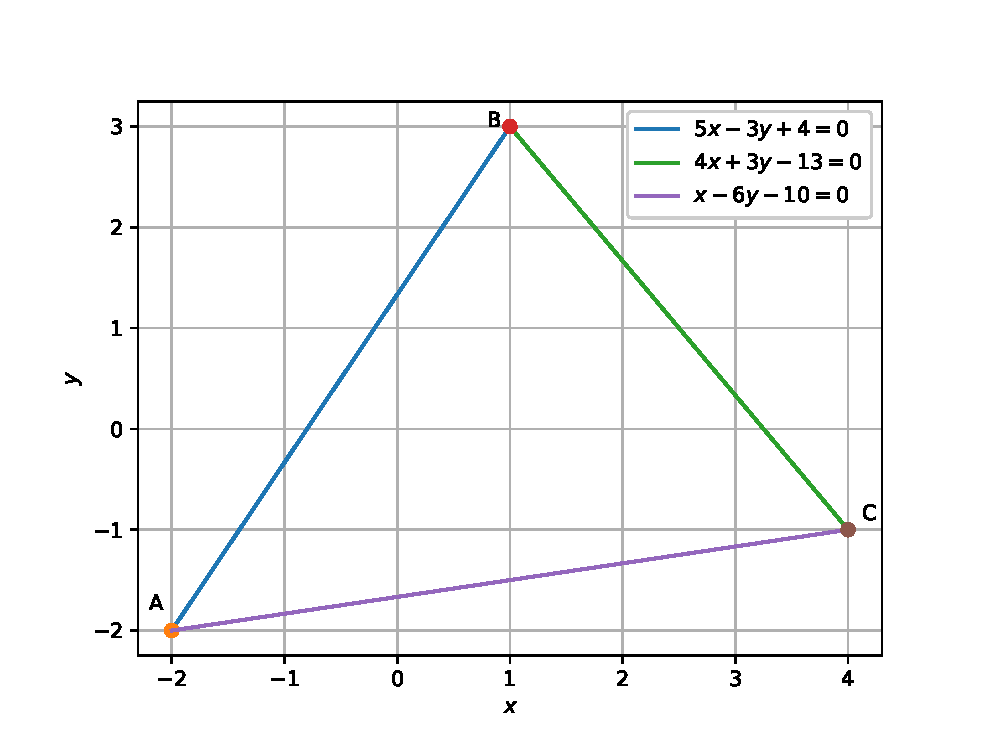
\includegraphics[width=\columnwidth]{./figs/triangle.eps}
\caption{}
\label{fig:triangle_def}
\end{figure}
%
\begin{problem}
\label{prob:line_eq}
Consider the line $AB$ with 
\begin{equation}
A =
\begin{pmatrix}
-2
\\
-2
\end{pmatrix},
B =
\begin{pmatrix}
1
\\
3
\end{pmatrix},
\end{equation}
%
If $AB$ is expressed by the equation
\begin{equation}
y = p_0x + p_1, 
\end{equation}
find $p_0$ and $p_1$.
%\begin{equation}
%p_0x + p_1y + p_2 = 0,
%\end{equation}
%find $p_0,p_1$ and $p_2$.
\end{problem}
\solution
Let
\begin{align}
A = 
\begin{pmatrix}
A_0
\\
A_1
\end{pmatrix},
B = 
\begin{pmatrix}
B_0
\\
B_1
\end{pmatrix},
\end{align}
%
The equation of $AB$ is given by
%
\begin{align}
\label{eq:line_two_pt}
\frac{y - A_1}{x-A_0} &= \frac{A_1 \! - \! B_1}{A_0 \! - \! B_0} 
\\
\implies  y &= \frac{A_1 \! - \! B_1}{A_0 \! - \! B_0} x + A_1 - A_0 \frac{A_1 \! - \! B_1}{A_0 \! - \! B_0}
\\
&= \frac{A_1 \! - \! B_1}{A_0 \! - \! B_0} x + \frac{A_0 B_1 - A_1B_0}{A_0 \! - \! B_0} 
%\implies \brak{A_1 - B_1}x &+ \brak{B_0-A_0}y + A_0B_1 - A_1 B_0 = 0
\label{eq:CA}
\end{align}
%
after some algebra. Thus,
\begin{align}
p_0 &= \frac{A_1 \! - \! B_1}{A_0 \! - \! B_0} 
\\
p_1 &= \frac{A_0 B_1 - A_1B_0}{A_0 \! - \! B_0} 
\end{align}

%\begin{equation}
%p_0 = A_1 - B_1, p_1 = B_0-A_0, p_2 = A_0B_1 - A_1 B_0.
%\end{equation}
The following python code computes the numerical values and the equation for $AB$ is
\begin{equation}
y =1.67x +1.33
%5x -3y +4 = 0
\end{equation}
\lstinputlisting{./codes/coeffs.py}
\begin{problem}
Let 
\begin{equation}
C =
\begin{pmatrix*}[r]
4
\\
-1
\end{pmatrix*}.
\end{equation}
%
Find the equations of $BC$ and $CA$
\end{problem}
%\solution
%The following code yields the coefficients resulting in the respective equations
%%
%\begin{align}
%4x + 3y -13 &= 0
%\\
%x - 6y - 10 &= 0
%\end{align}
%%
%\lstinputlisting{./codes/all_coeffs.py}
%\begin{problem}
%An alternative equation of the line $AB$ is
%\begin{equation}
%y = p_0x + p_1 
%\end{equation}
%%
%Find the equations of $AB,BC$ and $CA$.
%\end{problem}
%\solution From \eqref{eq:line_two_pt},
%\begin{align}
%p_0 &= \frac{A_1 \! - \! B_1}{A_0 \! - \! B_0} 
%\\
%p_1 &= A_1 - A_0\frac{A_1 \! - \! B_1}{A_0 \! - \! B_0} 
%\nonumber\\
%&= \frac{A_0 B_1 - A_1B_0}{A_0 \! - \! B_0} 
%\end{align}
%%
%The following python code calculates the above coefficients resulting in the equations for $AB,BC,CA$
%\begin{align}
%y &=1.67x +1.33
%\\
%y &=-1.33x + 4.33
%\\
%y &=0.16x -1.67
%\end{align}
%\begin{problem}
%Draw the lines $AB,BC$ and $CA$.
%\end{problem}
%
\section{Medians of a Triangle}
\begin{problem}
Find the coordinates of $D, E$ and $F$ of the mid points of $AB, BC$ and $CA$ respectively for  $\Delta ABC$. 
\end{problem} 
\solution
The coordinates of the mid points are given by
%
\begin{align}
D &= \frac{B+C}{2}, E = \frac{C+A}{2}, F = \frac{A+B}{2}
\end{align}
%
The following code computes the values resulting in
\begin{equation}
D = \begin{pmatrix}
2.5
\\
1
\end{pmatrix},
E = \begin{pmatrix}
1
\\
-1.5
\end{pmatrix},
F = \begin{pmatrix}
-0.5
\\
0.5
\end{pmatrix},
\end{equation}
\lstinputlisting{./codes/mid_points.py}
\begin{problem}
Find the equations of $AD,BE$ and $CF$. These lines are the {\em medians} of $\Delta ABC$
\end{problem}
\solution Use the code in Problem \ref{prob:line_eq}. 
%and simplifying, the respective equations are
%\begin{align}
%2x -3y-2 &=0
%\\
%x-1 &= 0
%\\
%x+3y-1 &=0
%\end{align}
%
\begin{problem}
\label{prob:median}
Find the point of intersection of $AD$ and $CF$.
\end{problem}
\solution
Let the respective equations  be
\begin{align}
y &= p_0x + p_1 \text{ and}
\\
y &= q_0x+q_1
%p_0 x + p_1 + p_2 &= 0
%\\
%q_0 x + q_1 + q_2 &= 0
\end{align}
This can be written as the matrix equation
\begin{equation}
\begin{pmatrix*}[r]
p_0 & -1 
\\
q_0 & -1 
\end{pmatrix*}
\begin{pmatrix}
x
\\
y
\end{pmatrix}
=-
\begin{pmatrix}
p_1
\\
q_1
\end{pmatrix}
\end{equation}
The following code yields the point of intersection 
\begin{equation}
G =
\begin{pmatrix}
1
\\
0
\end{pmatrix}
\end{equation}
\lstinputlisting{./codes/line_intersect.py}
\begin{problem}
Using the code in Problem \ref{prob:median}, verify that $G$ is the point of intersection of $BE,CF$ as well as
$AD,BE$.  $G$ is known as the {\em centroid} of $\Delta ABC$.
\end{problem}
\begin{problem}
Graphically show that the medians of $\Delta ABC$ meet at the centroid.
\end{problem}
\begin{problem}
Verify that
\begin{equation}
G = \frac{A+B+C}{3}
\end{equation}
\end{problem}
%\begin{problem}
%$AD, BE$ and $CF$ are defined to be the medians of $\Delta ABC$.  Draw them and verify that they meet at a point.
%\end{problem}
%\solution The following code results in Fig. \ref{fig:median_def}. Note that the medians meet at the {\em centroid} 
%\begin{equation}
%G = \frac{A+B+C}{3} = 
%\begin{pmatrix}
%1
%\\
%0
%\end{pmatrix}.
%\end{equation}
%\lstinputlisting{./figs/median_def.tex}
%\begin{figure}[!h]
%\centering
%\resizebox {\columnwidth} {!} {
%\input{./figs/median_def.tex}
%}
%\caption{Medians of $\Delta ABC$ meet at $G$.}
%\label{fig:median_def}
%\end{figure}
\section{Altitudes of a Triangle}
\begin{definition}
In $\Delta ABC$,  Let $P$ be a point on $BC$ such that $AP \perp BC$.  Then $AP$ is defined to be 
an {\em altitude} of $\Delta ABC$.
\end{definition}
\begin{problem}
\label{prob:alt_eq}
Find the equation of $AP$.
\end{problem}
\solution
Let the equation for $BC$ and $AP$ be
\begin{align}
y & = p_0x + p_1
\\
y & = q_0x + q_1
\end{align}
%
respectively. Since, $AP \perp BC$,
\begin{equation}
p_0q_0 = -1
\end{equation}
%
The equation for $AP$ is then obtained as
%
\begin{align}
y - A_1 &= q_0\brak{x - A_0}
\\
\implies y &= q_0 x + A_1 - q_0 A_0
\end{align}
%
From the following python code, $AP$ can be expressed as
%
\begin{equation}
y = 0.75x - 0.5
\end{equation}
%
\lstinputlisting{./codes/alt_eq.py}
%
\begin{problem}
Find the equations of the altitudes $BQ$ and $CR$. 
\end{problem}
\solution 
Using the code in Problem \ref{prob:alt_eq}, the respective equations are
\begin{align}
y &= -6x + 9
\\
y &= -0.6x + 1.4
\end{align}
%
\begin{problem}
Find the point of intersection of $AP$ and $BQ$.
\end{problem}
\solution Using the code in Problem \ref{prob:median}, the desired point of intersection is
%
\begin{equation}
H = 
\begin{pmatrix}
 1.407
 \\
 0.56
\end{pmatrix}
\end{equation}
%
Interestingly, $BQ$ and $CR$ also intersect at the same point.  Thus, the altitudes of a triangle
meet at a single point known as the {\em orthocentre}
%
\begin{problem}
Find $P,Q,R$.
\end{problem}
\solution $P$ is the intersection of $AP$ and $BC$.  Thus, the code in Problem \ref{prob:median} can be used to find 
$P$.  The desired coordinates are
%
\begin{align}
P =
\begin{pmatrix}
 2.32
 \\
  1.24
\end{pmatrix}
,
Q=
\begin{pmatrix}
 1.73
 \\
 -1.38
\end{pmatrix},
R=
\begin{pmatrix}
 0.03
 \\
  1.38
\end{pmatrix}
\end{align}
%
\begin{problem}
Draw $AP, BQ$ and $CR$ and verify that they meet at $H$.  
\end{problem}
\section{Angle Bisectors of a Triangle}
%
\begin{definition}
In $\Delta ABC$, let $U$ be a point on $BC$ such that $\angle BAU = \angle CAU$. Then $AU$ is known as the {\em angle bisector}.
\end{definition}
\begin{problem}
Find the length of $AB,BC$ and $CA$
\end{problem}
\solution The length of $CA$ is given by
\begin{align}
CA = \sqrt{\brak{C_0-A_0}^2 + \brak{C_1 - A_1}^2}
%&= \sqrt{37}.
\end{align}
The following code calculates the respective values as
%
\begin{equation}
AB =  5.83, BC =  5, CA =  6.08
\end{equation}
%
\lstinputlisting{./codes/side_length.py}
\begin{problem}
If $AU,BV$ and $CW$ are the angle bisectors, find the coordinates of $U,V$ and $W$.
\end{problem}
\solution Using the section formula,
\begin{align}
W &= \frac{AW.B+WB.A}{AW + WB} = \frac{\frac{AW}{WB}.B+A}{\frac{AW}{WB} + 1}
\\
&= \frac{\frac{CA}{BC}.B+A}{\frac{CA}{BC} + 1}
\\
&= \frac{{CA}\times B+{BC}\times A}{{BC} + {CA}}
\\
&= \frac{a\times A + b\times B}{a + b}
\end{align}
where $a = BC, b = CA$, 
since the angle bisector has the property that
%
\begin{equation}
\frac{AW}{WB} = \frac{CA}{AB}
\end{equation}
%
The following code computes the coordinates as
\begin{align}
U=
\begin{pmatrix}
2.47
\\
1.04
\end{pmatrix},
V =
\begin{pmatrix*}[r]
1.23
\\
-1.46
\end{pmatrix*}
& \approx 
\begin{pmatrix*}[r]
-0.35
\\
0.75
\end{pmatrix*} 
\end{align}
%
\lstinputlisting{./codes/angle_bisect_coord.py}
\begin{problem}
Find the intersection of $AU$ and $BV$.% and $CW$ and verify that they meet at a point $I$.  
\end{problem}
\solution Using the code in Problem \ref{prob:median}, the desired point of intersection is
\begin{equation}
I = 
\begin{pmatrix}
1.15
\\
0.14
\end{pmatrix}
\end{equation}
%
It is easy to verify that even $BV$ and $CW$ meet at the same point.  $I$ is known as
the {\em incentre} of $\Delta ABC$. 
\begin{problem}
Draw $AU, BV$ and $CW$ and verify that they meet at a point $I$.  
\end{problem}
%\solution The following code results in Fig. \ref{fig:bisect_def}. Note that the angle bisectors meet at the {\em incentre} $I$.
%\lstinputlisting{./figs/bisect_def.tex}
%\begin{figure}[!h]
%\centering
%\resizebox {\columnwidth} {!} {
%\input{./figs/bisect_def.tex}
%}
%\caption{Angle bisectors of $\Delta ABC$ meet at $I$.}
%\label{fig:bisect_def}
%\end{figure}
%%
\begin{problem}
Verify that
\begin{align}
I = \frac{BC.A + CA.B + AB.C}{AB+BC+CA}
\end{align}
%
\end{problem}
\begin{problem}
\label{prob:incircle_normal}
Let the perpendiculars from $I$ to $AB, BC$ and $CA$ be $IX, IY, IZ$.  Verify that
\begin{equation}
IX = IY = IZ = r
\end{equation}
$r$ is known as the {\em inradius} of $\Delta ABC$.
\end{problem}
\solution
The distance of a point $\brak{a,b}$ from the line $y = p_0x+p_1$ is given by 
\begin{equation}
\frac{\abs{ap_0-b+p_1}}{\sqrt{p_0^2+1}}
\end{equation}
The following code computes IX.
\lstinputlisting{./codes/inradius.py}
\section{Circle}

\begin{definition}
From Problem \ref{prob:incircle_normal}, it is obvious that  a circle with centre at $I$ and radius $r$ passing through $X, Y, Z$ can be drawn.  
The {\em incircle} is defined as the circle with centre at the incentre I and radius equal to the inradius.
\end{definition}
\begin{problem}
\label{prob:incircle}
Obtain the equation of the incircle of $\Delta ABC$ and draw it.
\end{problem}
%
\solution Letting $I = \brak{a,b}$, the equation of the incircle is given by
%
\begin{equation}
\brak{x-a}^2 + \brak{y-b}^2 = r^2,
\end{equation}
%
where $r$ is the inradius.  The following code plots this circle in Fig. \ref{fig:incircle}
\lstinputlisting{./codes/In_circle.py}
\begin{figure}[!h]
\centering
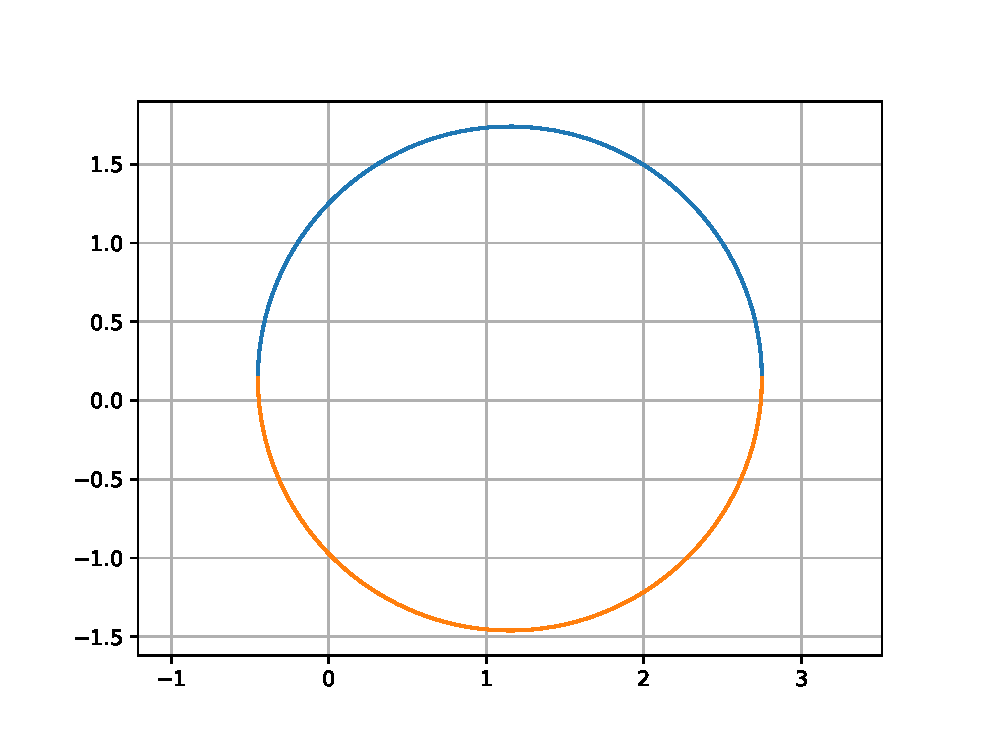
\includegraphics[width=\columnwidth]{./figs/incircle.eps}
\caption{}
\label{fig:incircle}
\end{figure}
%

\section{Tangent and Derivative}
\begin{definition}
A line that meets the circle at exactly one point is known as a {\em tangent} to the circle.
\end{definition}
%
\begin{problem}
Draw $\Delta ABC$ and its incircle in the same graph and verify that the lines $AB, BC, CA$ are tangents to the incircle 
\end{problem}
\solution Fig. \ref{fig:tri_incircle} can be drawn using the codes in Problems \ref{prob:draw_triangle} and \ref{prob:incircle}.  It is obvious
from the figure that $AB,BC$ and $CA$ are tangents to the incircle.
%
\begin{figure}[!h]
\centering
\includegraphics[width=\columnwidth]{./figs/tri_incircle.eps}
\caption{}
\label{fig:tri_incircle}
\end{figure}
%
\begin{problem}
Let the equation of $AB$ be 
\begin{equation}
p_0x+p_1y+p_2 = 0
\end{equation}
%
and the incircle be
\begin{equation}
\brak{x-a}^2 + \brak{y-b}^2 = r^2,
\end{equation}
Verify that
\begin{multline}
\sbrak{p_0\brak{p_2+bp_1}-ap_1^2}^2 
\\
= \brak{p_0^2+p_1^2}\sbrak{p_1^2a^2+\brak{p_2+bp_1}^2-p_1^2r^2}
\end{multline}
and the point of contact 
\begin{equation}
X =
\begin{pmatrix}
\frac{ap_1^2-p_0\brak{p_2+bp_1}}{p_0^2+p_1^2}
\\
-\frac{p_2}{p_1}+\frac{p_0}{p_1}\frac{ap_1^2-p_0\brak{p_2+bp_1}}{p_0^2+p_1^2}
\end{pmatrix}
\end{equation} 
\end{problem}
\solution
The following code computes the point of contact 
\lstinputlisting{./codes/tangent_poc.py}
\begin{problem}
Verify that
\begin{align}
AX = AZ
\\
BX = BY
\\
CY = CZ
\end{align}
\end{problem}
\begin{problem}
Devise a method for calculating the slope of the tangent at $X$, given the equation of the circle and the point $X$.
\end{problem}
\solution In Fig. \ref{fig:derivative}, it can be seen that the tangent at $X$ has the same slope as the chord $BC$.
From the equation of the circle, 
\begin{align}
(p_{1}-a)^{2}+(q_{1} -b)^{2} =r^{2}   
\\
(p_{2}-a) ^{2}+(q_{2} -b)^{2} =r^{2}  
\end{align}
which, after simplification, leads to the slope of the chord as
\begin{align}
\frac{q _{1}-q_{2}}{p_{1}-p_{2}}  &=  -\frac{p_{1}+p_{2}-2a}{q_{1}+q_{2}-2b}
\\
\Rightarrow \frac{\Delta y}{\Delta x}  &=  -\frac{p_{1}+p_{2}-2a}{q_{1}+q_{2}-2b}
\end{align}
%
If we keep choosing smaller chords parallel to $BC$, $p_1$ and $p_2$ come closer while $q_1$ and $q_2$ come closer, without
any change in the slope on the LHS.  The limiting behaviour results in $p_1=p_2=p$ and $q_1=q_2=q$.  This results
in an expression for the slope of the tangent at $X$
\begin{equation}
\frac{dy}{dx}=-\frac{{p}-{a}}{{q}-{b}}
\end{equation}
where
\begin{equation}
\lim_{\Delta x \rightarrow 0} \frac{\Delta y}{\Delta x} = \frac{dy}{dx}.
\end{equation}
\begin{figure}[!h]
\centering
\resizebox {\columnwidth} {!} {
\input{./figs/derivative.tex}
}
\caption{Notion of the derivative.}
\label{fig:derivative}
\end{figure}
%
\begin{problem}
Verify that the derivative of the circle at $X$ is actually the slope of $AB$.
\end{problem}
%
\solution The verificaton is done by the following program.
\lstinputlisting{./codes/derivatives.py}
\section{Conic Sections}
\begin{problem}
\label{prob:unit_circle}
Plot the circle 
\begin{equation}
\label{eq:unit_circle}
x^2+y^2=1
\end{equation}
\end{problem}
\solution
\lstinputlisting{./codes/unit_circle.py}
\begin{problem}
Show that \eqref{eq:unit_circle} can be expressed as
\begin{equation}
\begin{pmatrix}
x & y & 1
\end{pmatrix}
\begin{pmatrix}
1 & 0 & 0
\\
0 & 1 & 0
\\
0 & 0 & -1
\end{pmatrix}
\begin{pmatrix}
x
\\
y
\\
1
\end{pmatrix}
= 0
\end{equation}
\end{problem}
\begin{problem}
\label{prob:circle_parabola}
Show that
\begin{equation}
\begin{pmatrix}
x & y & 1
\end{pmatrix}
M^{T}
\begin{pmatrix}
1 & 0 & 0
\\
0 & 1 & 0
\\
0 & 0 & -1
\end{pmatrix}
M
\begin{pmatrix}
x
\\
y
\\
1
\end{pmatrix}
= 0
\end{equation}
for
\begin{equation}
M = 
\begin{pmatrix}
2 & 1 & 0
\\
1 & 1 & 0
\\
2 & 1 & 1
\end{pmatrix}
\end{equation}
can be expressed as
\begin{equation}
\label{eq:parabola_projection}
x^2+2xy+y^2 - 4x - 2y -1 = 0	
\end{equation}
\end{problem}
\begin{problem}
Show that \eqref{eq:parabola_projection} results in the curve in Fig. \ref{fig:parabola_projection}.  This is known as a parabola.
\end{problem}
\begin{figure}[!h]
\centering
\includegraphics[width=\columnwidth]{./figs/parabola_projection.eps}
\caption{}
\label{fig:parabola_projection}
\end{figure}
%
\begin{problem}
Show that using  
\begin{equation}
M = 
\begin{pmatrix}
1 & 0 & 0
\\
0 & 0 & 1
\\
0 & 1 & 0
\end{pmatrix}
\end{equation}
in Problem \ref{prob:circle_parabola} results in 
\begin{equation}
\label{eq:hyperbola}
y^2-x^2 = 1
\end{equation}
\end{problem}
\begin{problem}
Sketch \eqref{eq:hyperbola} to obtain Fig. \ref{fig:circle_hyperbola}.
This curve is known as a {\em hyperbola}
\end{problem}
\solution	
\lstinputlisting{./codes/circle_hyperbola.py}
\begin{figure}[!h]
\centering
\includegraphics[width=\columnwidth]{./figs/circle_hyperbola.eps}
\caption{}
\label{fig:circle_hyperbola}
\end{figure}

\begin{problem}
Generate the points 
\begin{equation}
\begin{pmatrix}
x_1
\\y_1
\end{pmatrix}
=
M \begin{pmatrix}
x
\\y
\end{pmatrix}
\end{equation}
where $x,y$ are the points generated in Problem \ref{prob:unit_circle}. Plot $y_1$ with respect to $x_1$.
The figure that you obtain in Fig. \ref{fig:ellipse_transform} is known as an {\em ellipse}.
\end{problem}
\solution
\lstinputlisting{./codes/circle_ellipse.py}
\begin{figure}[!h]
\centering
\includegraphics[width=\columnwidth]{./figs/ellipse_transform.eps}
\caption{}
\label{fig:ellipse_transform}
\end{figure}
%
\begin{problem}
Draw the curve
\begin{equation}
\label{eq:ellipse}
\frac{x^2}{9}+\frac{y^2}{4} = 1
\end{equation}
\end{problem}
Comment.
\section{Area Within a Parabola}
\begin{problem}
Sketch the parabola
\begin{equation}
y^2 = x
\end{equation}
\end{problem}
%
\begin{problem}
\label{prob:parabola_area}
Using $n$ rectangles of equal width as shown in Fig. \ref{fig:parabola_area}, find the limting area of the parabola in
$x \in \brak{0,1}$.
\end{problem}
\begin{figure}[!h]
\centering
\includegraphics[width=\columnwidth]{./figs/parabola_area.eps}
\caption{}
\label{fig:parabola_area}
\end{figure}
%
\solution Considering the width of the rectangle as $h = \frac{1}{n}, n = 100$, the approximate area of the parabola
can be computed as
%
\begin{align}
A &= h*\brak{\sqrt{h}+\sqrt{2h}+\dots+\sqrt{100h}}
\\
&\approx 0.67
\end{align}
using the following program
\lstinputlisting{./codes/parabola_area.py}
%
\subsection{Arithmetic Progression}
\begin{problem}
\label{prob:parabola_area}
Plot
\begin{equation}
\label{eq:parabola_area}
y = x^2
\end{equation}
%
and verify that the area under this parabola for $x \in \brak{0,1}$ is $A_0=1-A$.
\end{problem}
%
\solution
\begin{figure}[!h]
\centering
\includegraphics[width=\columnwidth]{./figs/parabola_inverted_area.eps}
\caption{}
\label{fig:parabola_inverted_area}
\end{figure}
%
The following code
%
\lstinputlisting{./codes/parabola_inverted_area.py}
%
yields the area in Fig.\ref{fig:parabola_inverted_area} as $A_0\approx 0.33 = 1 - A = 1 - 0.67$.
\begin{problem}
Show that the limiting area in Problem \ref{prob:parabola_area} is
\begin{equation}
A_0 = \lim_{n\to \infty}\brak{\frac{1}{n}}^3\sum_{k=1}^{n}k^2 = \frac{1}{3}
\end{equation}
\end{problem}
\solution 
%
We have
\begin{align}
k^3 - \brak{k-1}^3 &= 3k^2-3k + 1
\\
\Rightarrow n^3  &= 3\sum_{k=1}^{n}k^2-3\sum_{k=1}^{n}k + n
\\
\Rightarrow \sum_{k=1}^{n}k^2 & = \frac{1}{3}\sbrak{n^3 + 3\sum_{k=1}^{n}k - n}
\end{align}
%
Letting
\begin{align}
S_n &= 1 + 2 + \dots +n
\\
S_n &= n + n-1 + \dots +1
\\
\Rightarrow 2S_n &= n\brak{n+1}
\\
\Rightarrow S_n &= \frac{n\brak{n+1}}{2}
\end{align}
Thus,
\begin{align}
\sum_{k=1}^{n}k^2 & = \frac{1}{3}\sbrak{n^3 + 3 \frac{n\brak{n+1}}{2} - n}
\\
& = \frac{n}{6}\sbrak{2n^2 + 3n + 1}
\\
&=\frac{n\brak{n+1}\brak{2n+1}}{6}
\end{align}
and
\begin{align}
A_0 &= \lim_{n\to \infty}\brak{\frac{1}{n}}^3\sum_{k=1}^{n}k^2 
\\
&= \lim_{n\to \infty}\frac{1}{6}\brak{1+\frac{1}{n}}\brak{2+\frac{1}{n}}
\\
&= \frac{1}{3}
\end{align}
%
This process of finding the area under a curve is known as {\em integration}.  Integration
is the opposite of differentiation. The sequence that is summed in $S_n$ is known as an 
{\em Arithmetic Progression}.
\subsection{Geometric Progression}
\begin{problem}
Plot the parabola
%
\begin{equation}
y = x^2
\end{equation}
%
for $x\in\brak{0,1}$ with points $\brak{r^k,0}, k = 0,1,\dots,n$ for $r = 0.8, n = 10$.
\end{problem}
\solution
The following code
%
\lstinputlisting{./codes/parabola_hist_gp.py}
%
plots Fig. \ref{fig:parabola_area_gp}
\begin{figure}[!h]
\centering
\includegraphics[width=\columnwidth]{./figs/parabola_area_gp.eps}
\caption{}
\label{fig:parabola_area_gp}
\end{figure}
%
\begin{problem}
Calculate the area of the parabola using Fig. \ref{fig:parabola_area_gp} with $n = 100, r = 0.98$.
\end{problem}
\solution 
The intervals are of width $r^{k-1}\brak{1-r}, k = 1, \dots, n$.  The corresponding heights are $r^{2k-2}$.  Thus, the area is
%
\begin{align}
A_0 &= \sum_{k=1}^{n}r^{k-1}\brak{1-r}r^{2k-2}
\\
&=\brak{1-r}\sum_{k=1}^{n}r^{3k-3}
\end{align}
%
The following code calculates the desired area as 0.33
\lstinputlisting{./codes/parabola_area_gp.py}
\begin{problem}
Obtain the area in the previous problem as the limit of a sum.
\end{problem}
\solution Let 
\begin{align}
\label{eq:parabola_area_gp}
A_0 &= \lim_{\substack{r \to 1 \\ n \to \infty}}\brak{1-r}\sum_{k=1}^{n}r^{3k-3}, \quad r < 1
\end{align}
If $p = r^3$,
\begin{align}
S_n &= \sum_{k=1}^{n}p^{k-1}
\\
\Rightarrow pS_n &= \sum_{k=1}^{n}p^{k}
\\
\Rightarrow \brak{1-p}S_n &= 1 - p^{n}
\\
\Rightarrow S_n &= \frac{1-p^n}{1-p} 
\end{align}
The sequence $p^{k-1}, k = 1, \dots, n$ is known as a {\em Geometric Progression}.  Substituting in \eqref{eq:parabola_area_gp},
%
\begin{align}
A_0 &= \lim_{\substack{r \to 1 \\ n \to \infty}}\brak{1-r}\frac{1-r^{3n}}{1-r^3}
\\
&= \lim_{\substack{r \to 1 \\ n \to \infty}}\frac{1-r^{3n}}{1+r+r^2}
\\
&= \frac{1}{3} \quad \brak{\because r^{3n} \to 0}
\end{align}
\end{document}


